\documentclass[a4paper,12pt]{article}
%%%%%%%%%%%%%%%%%%%%%%%%%%%%%%%%%%%%%%%%%%%%%%%%%%%%%%%%%%%%%%%%%%%%%%%%%%%%%%%%%%%%%%%%%%%%%%%%%%%%%%%%%%%%%%%%%%%%%%%%%%%%%%%%%%%%%%%%%%%%%%%%%%%%%%%%%%%%%%%%%%%%%%%%%%%%%%%%%%%%%%%%%%%%%%%%%%%%%%%%%%%%%%%%%%%%%%%%%%%%%%%%%%%%%%%%%%%%%%%%%%%%%%%%%%%%
\usepackage{eurosym}
\usepackage{vmargin}
\usepackage{amsmath}
\usepackage{graphics}
\usepackage{epsfig}
\usepackage{subfigure}
\usepackage{fancyhdr}
%\usepackage{listings}
\usepackage{framed}
\usepackage{graphicx}

\setcounter{MaxMatrixCols}{10}
%TCIDATA{OutputFilter=LATEX.DLL}
%TCIDATA{Version=5.00.0.2570}
%TCIDATA{<META NAME="SaveForMode" CONTENT="1">}
%TCIDATA{LastRevised=Wednesday, February 23, 2011 13:24:34}
%TCIDATA{<META NAME="GraphicsSave" CONTENT="32">}
%TCIDATA{Language=American English}

\pagestyle{fancy}
\setmarginsrb{20mm}{0mm}{20mm}{25mm}{12mm}{11mm}{0mm}{11mm}
\lhead{Quality Control in R - Drew Conway} \rhead{edited : Kevin O'Brien}
%\chead{Dublin R}


\begin{document}
\tableofcontents

\newpage
% http://blog.yhathq.com/posts/quality-control-in-r.html
% http://support.sas.com/rnd/app/qc/papers/spcsugi94.pdf
\section{Quality Control in R - Drew Conway}

\begin{itemize}
\item Quality Control and quality assurance are important functions in most businesses from manufacturing to software development. For most, this means that one or more people are meticulously inspecting what's coming out of the factory, looking for imperfections and validating that requirements for products and services produced are satisfied. 

\item Often times QC and QA are performed manually by a select few specialists, and determining suitable quality can be extremely complex and error-prone.
\item 
This is a post about quality assurance automation using statistics and \texttt{R}.
\end{itemize}
\newpage
\subsection{What is statistical quality control?}
\begin{itemize}
\item Statistical quality control is a quantitative approach to monitoring and controling a process. The best way to explain it is though an example.

\item  Suppose you're the manager at a factory that manufactures lug nuts. And let's suppose your 10 mm long lug nuts continue to function within a 10 percent margin of error (i.e. customers have a tolerance for error of roughly +/- 1 mm in length). 

\item As long as your producing lug nuts measuring between 9 and 11 mm in length, you'd consider your machine to be functioning as designed.

\item  How would you know if your machine has suffered a malfunction? A 9.7mm lug nut could be the sign that your machine is producing lug nuts that are too small, or it could just be natural error that occurs for a machine that's supposed to make 10mm lug nuts.

\item  Take a look at the plots below. Can you tell which one has experienced a change in the mean?
\end{itemize}
\begin{figure}[h!]
\centering
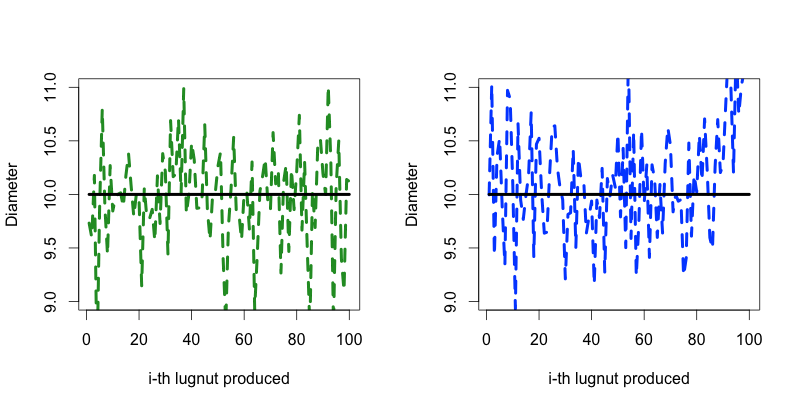
\includegraphics[width=0.99\linewidth]{./sqcr1}
\caption{}
\label{fig:sqcr1}
\end{figure}
%----------------------------------------------------- %
\newpage
\subsection{Framing the Problem}
\begin{itemize}
\item As a smart manager, you're using statistical quality control to identify issues with your machine. You can think of each lug nut as an observation. 
\item Since we're trying to make 10 mm lug nuts, we will assume that the mean lug nut (lug nut) is 10 mm. This means that over time, the mean lug nut diameter should approach 10 mm. 
\item We're also going to assume that our machine's mistakes are normally distributed which in our case means that more lug nuts are much more likely to be closer to 10 mm than farther away from it.
\end{itemize}
\newpage
\subsection{The qcc package}
\begin{itemize}
\item So we've come up with a good framework for our problem, now what?. Enter the \textbf{qcc} package in \texttt{R}. qcc is a library for statistical quality control. This magical little library was built by Luca Scrucca for nothing but statistical quality control. 
\item qcc is extremely easy to use. You provide it with data and it tells you which points are considered to be outliers based on the \textit{Shewart Rules}. 
\item It even color codes them based on how irregular each point is. 
\item In the example below you can see that for the last 10 points of the 2nd dataset I shifted the mean of the data from 10 to 11.
\end{itemize}
\subsubsection{Background}
\begin{itemize}
\item Back in the 1950s, the now defunct Western Electric Company was looking for a better way to detect problems with telephone and eletrical lines. They came up with a set of rules to help them identify problematic lines. 
\item While you might not be monitoring telephone lines, \textbf{qcc} can help you monitor transaction volumes, visitors or logins on your website, database operations, and lots of other processes.
\item The rules look at the historical mean of a series of datapoints and based on the standard deviation, the rules help judge whether a new set of points is experiencing a mean shift.
\item The classic example is monitoring a machine that produces lug nuts. Let's say the machine is supposed to produce 2.5 inch long lug nuts. We measure a series of lug nuts with the following measurements: \[2.48, 2.47, 2.51, 2.52, 2.54, 2.42, 2.52, 2.58, 2.51.\] Is the machine broken? Well it's hard to tell, but the Western Electric Rules can help.

\item You can also define training/test set from within \textbf{qcc}. Simply add the data you want to calibrate it with as the first parameter, then add the parameter \texttt{newdata} with your test data (see code above and plot below).


\item Some processes might not be have normally distributed errors, but I've found that there are often ways in which you can transform your error term to make it behave normally. It all just depends on how creative you are.
\end{itemize}
\newpage

%# series of value w/ mean of 10 with a little random noise added in
%x <- rep(10, 100) + rnorm(100)
%# a test series w/ a mean of 11
%new.x <- rep(11, 15) + rnorm(15)
%# qcc will flag the new points
%qcc(x, newdata=new.x, type="xbar.one")
%view rawqcc_example.R hosted with ❤ by GitHub


EDIT : CHANGE THIS
\begin{framed}
\begin{verbatim}
library(qcc)
#make 2 plots in 1 figure
par(mfrow=c(1,2))
 
#points have base value of 10 w/ normally distributed error
lugnuts <- rep(10, 100) + rnorm(100, mean=0, sd=0.5)
qcc(lugnuts, type="xbar.one", center=10, add.stats=FALSE,
    title="1st Batch", xlab="i-th lugnut produced")
 
#first 90 points have base value of 10 w/ normally distributed error,
#last 10 points have base value of 11 w/ normally distributed error
lugnuts <- c(rep(10, 90), rep(11, 10)) + rnorm(100, mean=0, sd=0.5)
qcc(lugnuts, type="xbar.one", center=10, add.stats=FALSE,
    title="2nd Batch", xlab="i-th lugnut produced")
 
#example using holdout/test sets
lugnuts <- rep(10, 100) + rnorm(100, mean=0, sd=0.5)
qcc(lugnuts, newdata=rep(11, 10) + rnorm(10, mean=0, sd=0.5),
    type="xbar.one", center=10, add.stats=FALSE, title="2nd Batch", xlab="i-th lugnut produced")
\end{verbatim}
\end{framed}



\begin{figure}[h!]
\centering
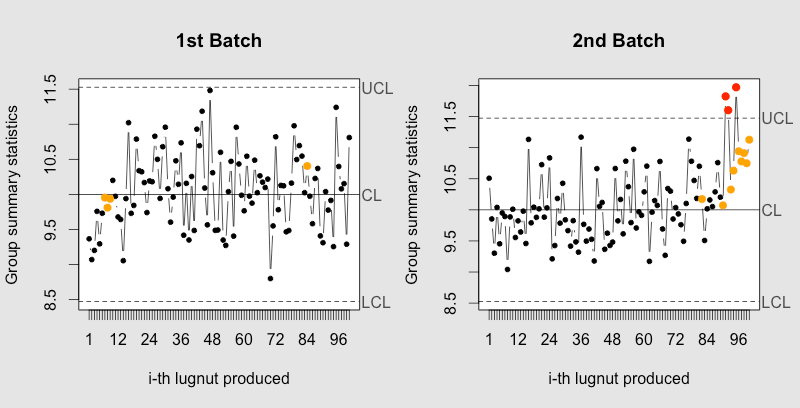
\includegraphics[width=0.7\linewidth]{./sqcr2}
\caption{}
\label{fig:sqcr2}
\end{figure}
\newpage
\subsection{Building Your Own Quality Control Charts}
\begin{itemize}
\item As great as \textbf{qcc} is, it doesn't have my favorite type of statistical qualtiy control - The Western Electric Rules (WER). The WER were first used by the \textit{Western Eletric Company} as a way to standardize how their employees monitored their eletric lines. 

\item While the Western Eletric Co. isn't around anymore, the rules they came up with are still really useful for monitoring processes. In a minute we'll show you how to implement them yourself, but first let's explain how they work.

\item The WER are remarkably straightforward and intuitive. For a recurring process take a sampling of points and measure the mean and the standard deviation. We'll use the mean as the "\textit{\textbf{center-line}}". Then create 3 zones above and below the center-line, each 1 standard deviation in width.


\item Based on these zones, the Western Eletric Co. came up with a set of rules to determine if a process is broken:
\end{itemize}
\begin{itemize}
\item One point lies beyond Zones +/- 3
\item 2 out of 3 consecutive points lie in Zone +/- 3 (and on the same side of the center-line)
\item 4 out of 5 consecutive points lie beyond the Zone +/- 2 (and on the same side of the center-line)
\item 8 consecutive points lie one the same side of the cetner-line
\end{itemize}

\newpage
\subsection{Implementing them on your own}
Despite how cool the WER are, they aren't in the qcc package. Luckly, with \texttt{R} they shouldn't be too tricky to implement ourselves.

\begin{figure}[h!]
\centering
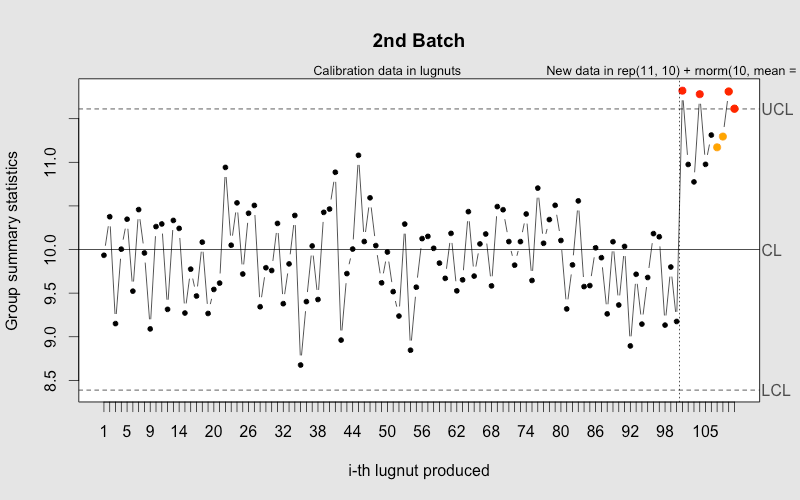
\includegraphics[width=0.7\linewidth]{./sqcr3}
\caption{}
\label{fig:sqcr3}
\end{figure}

\subsection{Defining the Zone}

The first thing we need to do is define the thresholds for each of the zones. Each zone is one standard deviation in width and there are 3 zones on each side of the center-line. Since we also want to know what the top/bottom of Zone +/- 3 is, we'll need to calculate 8 zones. What we end up with is a grid. The numbers in columns 1 and 2 correspond with the boundaries for Zone -3, columns 2 and 3 correspond with Zone -2, etc.
\begin{framed}
\begin{verbatim}
find_zones <- function(x) {
  x.mean <- mean(x)
  x.sd <- sd(x)
  boundaries <- seq(-4, 4)
  # creates a set of zones for each point in x
  zones <- sapply(boundaries, function(i) {
    i * rep(x.sd, length(x))
  })
  zones + x.mean
}
 
\end{verbatim}
\end{framed} 
\begin{verbatim}
head(find_zones(x))
# [,1]  [,2]  [,3]  [,4]  [,5]  [,6]  [,7]  [,8]  [,9]
# [1,] 7.954 8.493 9.032 9.572 10.11 10.65 11.19 11.73 12.27
# [2,] 7.954 8.493 9.032 9.572 10.11 10.65 11.19 11.73 12.27
# [3,] 7.954 8.493 9.032 9.572 10.11 10.65 11.19 11.73 12.27
# [4,] 7.954 8.493 9.032 9.572 10.11 10.65 11.19 11.73 12.27
# [5,] 7.954 8.493 9.032 9.572 10.11 10.65 11.19 11.73 12.27
# [6,] 7.954 8.493 9.032 9.572 10.11 10.65 11.19 11.73 12.27
\end{verbatim}
%----------------------------------------------------------%
\newpage
\section{Finding Outliers}

Since we know what the range is for each zone, now we need to determine which zone every point falls in. First we're going to compare our points to each zone by using x > zones. This gives us a giant matrix of TRUE/FALSE values. We can then use this to calculate the zone that each point falls into by summing the rows (TRUE/FALSE evaluates to 1/0 when summed). We can use rowSums which does rowise summation on a data.frame/matrix. The value of each item is the zone which it belongs in plus 4 (the extra 4 is because a value of 1 maps to zone -3), so we subtract 4 from the vector and...voila we have the zone that each point falls into.

Once we've determined which zone a given point falls in, we can compute rules for each index within the group. If a given index violates a rule, we flag it with a +/- 1 (+ for zone above center-line, - for zone below center-line).

\begin{framed}
\begin{verbatim}
evaluate_zones <- function(x) {
  zones <- find_zones(x)
  colnames(zones) <- paste("zone", -4:4, sep="_")
  x.zones <- rowSums(x > zones) - 4
  x.zones
}
 
evaluate_zones(x)
# [1]  0  2  0  1  2  0  0  1 -1  0 -1  1  1  1 -2  1 ...
 
find_violations <- function(x.zones, i) {
  values <- x.zones[max(i-8, 1):i]
  rule4 <- ifelse(all(values > 0), 1,
                  ifelse(all(values < 0), -1,
                         0))
 
  values <- x.zones[max(i-5, 1):i]
  rule3 <- ifelse(sum(values >= 2) >= 4, 1,
                  ifelse(sum(values <= -2) >= 4, -1,
                         0))
  
  values <- x.zones[max(i-3, 1):i]
  rule2 <- ifelse(sum(values >= 3) >= 2, 1,
                  ifelse(sum(values <= -3) >= 2, -1,
                         0))
  
  values <- x.zones[i]
  rule1 <- ifelse(any(values > 3), 1,
                  ifelse(any(values < -3), -1,
                         0))
  
  c("rule1"=rule1, "rule2"=rule2, "rule3"=rule3, "rule4"=rule4)
}
 
find_violations(evaluate_zones(x), 70)
# rule1 rule2 rule3 rule4 
# 0     0     0     0 
\end{verbatim}
\end{framed}
%------------------------------------------------------------------------------------%
\newpage

\section{Putting them together}

Using the functions we've defined, we can now find compute the rules for each point adn then assign a color to any violations.
\begin{verbatim}

compute_violations <- function(x, start=1) {
  x.zones <- evaluate_zones(x)
  results <- ldply(start:length(x), function(i) {
    find_violations(x.zones, i)
  })
  results$color <- ifelse(results$rule1!=0, "pink",
                          ifelse(results$rule2!=0, "red",
                                 ifelse(results$rule3!=0, "orange",
                                        ifelse(results$rule4!=0, "yellow",
                                               "black"))))
  results
}
 
tail(compute_violations(x))
# rule1 rule2 rule3 rule4 color
# 95      0     1     1     0   red
# 96      1     1     1     0  pink
# 97      0     1     1     0   red
# 98      0     1     1     0   red
# 99      0     1     1     1   red
# 100     1     1     1     1  pink
\end{verbatim}
\newpage
\section{Visualizing It All}

With all of our datapoints, we can now make a quality control chart. We're going to use the original points and overaly them with the zones and then make each point the color of the rule if breaks (if any).
\begin{figure}
\centering
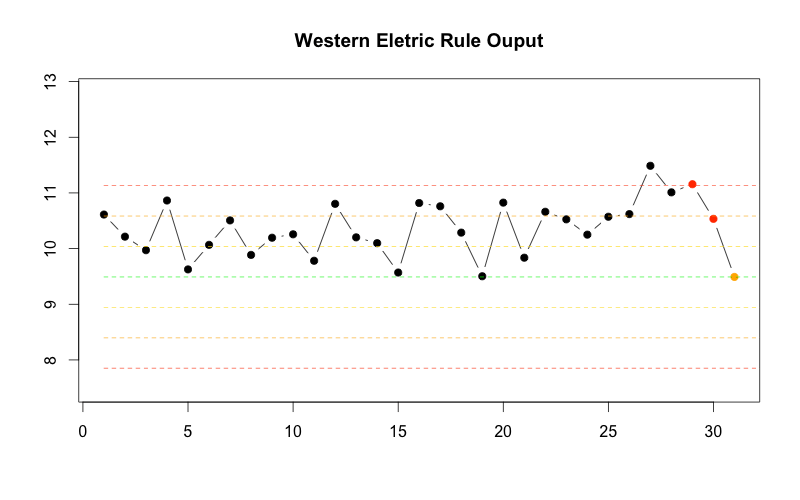
\includegraphics[width=0.7\linewidth]{./sqcr5}
\end{figure}

\begin{verbatim}
plot.wer <- function(x, holdout) {
  wer <- compute_violations(x, length(x) - holdout)
  bands <- find_zones(x)
  plot.data <- x[(length(x) - holdout):length(x)]
  plot(plot.data, col=wer$color, type='b', pch=19,
       ylim=c(min(bands), max(bands)),
       main="Western Eletric Rule Ouput",
       xlab="", ylab="")
  
  for (i in 1:7) {
    lines(bands[,i], col=cols[i], lwd=0.75, lty=2)
  }
}
 
x <- c(rep(10, 90), rep(10.5, 10)) + rnorm(100, mean=0, sd=0.5)
plot.wer(x, 30)
\end{verbatim}

\end{document}
Deploying to Yhat
Deploying this one is really easy. Since we've encapsulated most of the hard part into our helper functions, we just need to call compute_violations on our series of data. We can bypass the model.transform function since we're working with the raw data itself, and we don't have any external dependencies so we don't need to fill out model.require.

library(yhatr)
 
model.require <- function() {
  library(plyr)
}
 
model.transform <- function(df) {
  df
}
 
model.predict <- function(df) {
  data.frame(compute_violations(df$x))
}
 
yhat.config <- c(
  apikey="{YOUR APIKEY}",
  username="{YOUR USERNAME}"
)
yhat.deploy("westernElectricRules")
 
test <- data.frame(x=rnorm(100))
yhat.predict("westernElectricRules", 1, test)
view rawdeploy_wer.R hosted with ❤ by GitHub
Final Thoughts
Even though it's an old topic, statistical quality control is still highly relevant. While you might not be working at a lug nut factory, you probably have lots of jobs, processes, logs, or databse metric that you could monitor using control charts.
\end{document}
